\documentclass[a4paper, titlepage, headings=standardclasses, listof=totoc]{scrartcl}

%\usepackage{plex-serif}
\usepackage{csquotes}
\usepackage[hidelinks]{hyperref}
\usepackage[dutch]{babel}
\usepackage[backend=biber, citestyle=apa, style=apa]{biblatex}
\usepackage{graphicx}
\usepackage{xcolor}
\usepackage[shortlabels]{enumitem}
\usepackage[section]{placeins}
\usepackage{xltabular}
\usepackage{fancyhdr}
\usepackage{pdflscape}
\usepackage{svg}
\usepackage{caption}

% Bibliography.
\addbibresource{../Bibliografie.bib}

% Package used for adding header titles.
\let\origmaketitle\maketitle
\usepackage{titling}
\let\maketitle\origmaketitle

% Flips margins for two-sided prints.
\let\tmp\oddsidemargin
\let\oddsidemargin\evensidemargin
\let\evensidemargin\tmp
\reversemarginpar

% Chapter and title header.
\pagestyle{fancy}
\fancyhead[L]{\textsl{\leftmark}}
\fancyhead[R]{\textsc{\thetitle}}
\renewcommand{\footrulewidth}{0.4pt}

% Complementary colors to the red color from the HAN logo.
\definecolor{hanA}{HTML}{D91E57}
\definecolor{hanB}{HTML}{8C062E}
\definecolor{hanC}{HTML}{D9CD34}
\definecolor{hanD}{HTML}{09A9D9}
\definecolor{hanE}{HTML}{0D6F8C}

% Coloring elements.
%\let\HeadRule\headrule
%\let\FootRule\footrule
%\renewcommand\headrule{\color{hanE}\HeadRule}
%\renewcommand\footrule{\textcolor{hanE}\FootRule}
%\addtokomafont{section}{\color{hanA}}
%\addtokomafont{subsection}{\color{hanA}}
%\addtokomafont{subsubsection}{\color{hanA}}
%\let\oldtextbf\textbf
%\renewcommand{\textbf}[1]{\textcolor{hanB}{\oldtextbf{#1}}}

% Fonts.
%\renewcommand{\rmdefault}{bch}
\renewcommand{\rmdefault}{bch}
\renewcommand{\sfdefault}{qag}

% Custom commands and environments.
% Itemize without vertical spacing.
\newenvironment{smallitemize}{\begin{itemize}[nosep,after=\strut]}{\end{itemize}}
% Enumerate without vertical spacing.
\newenvironment{smallenumerate}{\begin{enumerate}[nosep,after=\strut]}{\end{enumerate}}
% Minipage made to look like a floating figure.
\newenvironment{mpfigure}{\vspace{\floatsep}\noindent\begin{minipage}{\linewidth}\captionsetup{type=figure}}{\end{minipage}\vspace{1.1\floatsep}}
\newcommand{\comment}[1]{}

% Custom title page entries.
\def\Version#1{\def\version{#1}}
\def\Subtitle#1{\def\csubtitle{#1}}
\def\Teacher#1{\def\teacher{#1}}

% Other settings.
\setlength{\LTpre}{0pt}

\newcounter{usecasestep}[subsection]
\newcommand{\usecasestep}[1]{\stepcounter{usecasestep}\theusecasestep.\:#1}

\newenvironment{usecasetable}
{
   \begin{xltabular}{\textwidth}{X}
}{
   \end{xltabular}
}

\newcommand{\startusecasetable}{\\\hline\endfirsthead\endhead\hspace*{\fill}\textit{Wordt vervolgd op de volgende pagina.} \\\hline\endfoot\endlastfoot}
\newcommand{\nextpart}{\\\hline}

\newcommand{\primaryactor}[1]{\textbf{Primaire actor:} #1}

\newenvironment{stakeholders}
{
   \noindent\begin{minipage}[t]{\linewidth}
      \textbf{Stakeholders en belangen:}
}
{
   \end{minipage}
}

\newenvironment{preconditions}
{
   \noindent\begin{minipage}[t]{\linewidth}
      \textbf{Precondities:}
}{
   \end{minipage}
}

\newenvironment{postconditions}
{
   \noindent\begin{minipage}[t]{\linewidth}
      \textbf{Postconditions:}
}{
   \end{minipage}
}

\newenvironment{basicflow}
{
   \noindent\begin{minipage}[t]{\linewidth}
      \textbf{Succesvol hoofdscenario:}\\
}{
   \end{minipage}
}

\newcommand{\basicflowheading}{\textbf{Actoractie} & \textbf{Systeemverantwoordelijkheid} \\\hline}

\newenvironment{alternativeflows}
{
   \noindent\begin{minipage}[t]{\linewidth}
      \textbf{Alternatieve scenario's:}\\
}{
   \end{minipage}
}

\title{Software Requirements Specification}
\Subtitle{OOSE OOAD casus - Quebble}
\Teacher{Marco Engelbart}
\Version{2}

\begin{document}

\begin{titlepage}
    \sffamily
    \begin{center}
    \vspace*{1cm}

    \color{hanA}\huge\textbf{\thetitle}
    
    \vspace{0.5cm}

    \color{hanB}\Large \csubtitle

    \vspace{1.5cm}\color{black}

    Sjoerd Scheffer

    \vspace{0.1cm}

    579392

    \vfill

    \includesvg{../Afbeeldingen/logo.svg}

    \vspace{2.0cm}\large

    Docent: \teacher

    \vspace{1.0cm}\normalsize

    \today

    \vspace{0.5cm}

    Versie \version
    
    \end{center}
\end{titlepage}
\cleardoublepage
\tableofcontents
\clearpage
\listoftables
\listoffigures
\clearpage


\clearpage\section{Inleiding}
%Introduction

\subsection{Algemene beschrijving}
%Overall description <Provide a short description of the software being specified and its purpose, including relevant benefits, objectives, and goals. If a separate description of the product scope is available (e.g. in the PvA), refer to it rather than duplicating its contents here.>
Het bedrijf Solid Games wil een quiz-applicatie Quebble ontwikkelen die beschikbaar wordt op de meest gangbare devices.

Een spel bestaat uit zowel open vragen als meerkeuzevragen, en de speler moet credits kopen om te kunnen spelen. De medewerkers van Solid Games zullen de quizzes beheren.

\subsection{Gebruikersklassen en karakteristieken}
%User classes and characteristics <Identify the various user classes (actors) that you anticipate will use this product. User classes may be differentiated based on the  subset of product functions used. Describe the pertinent characteristics of each user class. Certain requirements may pertain only to certain user classes. >
Deze sectie beschrijft de aanwezige actoren en hun relatie tot het eindproduct.
\begin{itemize}
   \item \textbf{Speler}: De eindgebruiker van het product. De speler kan het spel spelen door credits te gebruiken. De speler kan deze credits tegen vaste prijzen kopen in de applicatie.
   \item \textbf{Medewerker}: De medewerker die de quizzes en de bijbehorende vragen en antwoorden onderhoudt. De medewerker moet vragen aan het systeem kunnen toevoegen en verwijderen, en de sets aan vragen (quizzes) kunnen beheren.
\end{itemize}

\subsection{Werkomgeving}
%Operating environment <Describe the environment in which the software will operate, including the hardware platform, operating system and versions, and any other software components or applications with which it must peacefully coexist.>
Deze sectie beschrijft de omgeving waarin de applicatie functioneert.

De applicatie is aanvankelijk een console Java-applicatie voor desktop PC's.

Uiteindelijk draait de applicatie op PC's en mobiele telefoons. PC's en mobiele telefoons zijn namelijk de meest gangbare internetapparaten voor consumenten (\cite{globalstats}).

\subsection{Ontwerp- en implementatiebeperkingen}
%Design and implementation constraints <Describe any items or issues that will limit the options available to the developers. These might include: hardware (e.g. specific mobile platforms), specific technologies, tools, and databases to be used; interfaces to other applications; programming language required; or communications protocols>
Deze sectie beschrijft de beperkingen van het systeem die de opties van ontwikkelaars kunnen begrenzen.
\begin{itemize}
   \item De applicatie is in Java geschreven.
   \item De applicatie moet testbaar zijn doormiddel van unit tests.
   \item De applicatie moet aanvankelijk een console-applicatie zijn.
   \item De applicatie moet uiteindelijk als zowel desktop-applicatie als mobiele applicatie beschikbaar zijn.
   \item De applicatie gebruikt een in-memory object als mock voor een toekomstige database.
   \item De library waarmee de applicatie woorden controleert op correctheid moet vervangbaar zijn.
   \item De systematiek voor de puntentelling moet vervangbaar zijn.
\end{itemize}

\subsection{Productfuncties}
%Product functions <Summarize the major functions the product must perform or must let the user perform. Details will be provided in Section 3, so only a high level summary is needed here. In most cases, this section will primarily contain a use case diagram and brief use case descriptions >
Deze sectie bevat het usecasediagram en de korte usecasebeschrijvingen.

\begin{mpfigure}
   \centering
   \includegraphics[scale=0.7]{../Afbeeldingen/use case diagram.png}
   \caption{Usecasediagram}\label{fig:usecasediagram}
\end{mpfigure}

\noindent\begin{minipage}{\textwidth}
   De volgende korte beschrijven van de usecases uit figuur \ref{fig:usecasediagram} zijn volgens de methodiek van \textcite{larman} opgesteld \pnotecite[46]{larman}.
   \begin{itemize}
      \item \textbf{Registreren:} De speler voert een gebruikersnaam en wachtwoord in. Het systeem slaat de gegevens op, en wijst de speler 1000 credits toe.
      \item \textbf{Quiz spelen:} De speler start een quiz. Het systeem stelt vragen aan de speler. De speler beantwoordt een voor een de vragen. Het systeem geeft de speler een letter per goed antwoord. De speler maakt een woord van de letters. Het systeem controleert de antwoorden en het woord en kent de speler een score toe.
      \item \textbf{Credits bijkopen:} De speler kiest het aantal credits dat hij wil kopen. Het systeem geeft de bijbehorende prijs weer. De speler betaalt en het systeem kent de speler het gekozen aantal credits toe.
      \item \textbf{Quiz samenstellen:} De medewerker kiest 8 reeds opgeslagen actieve vragen. Het systeem slaat de vragen op in een speelbare quiz.
      \item \textbf{Quizvraag vervangen:} De medewerker kiest een reeds bestaande quiz. De medewerker kiest een vraag uit de quiz, en kiest vervolgens een vraag van buiten de quiz. Het systeem vervangt de geselecteerde quizvraag door de gekozen vraag van buiten de quiz.
      \item \textbf{Vraag toevoegen:} De medewerker vult een vraag en de bijbehorende categorie in. De medewerker geeft aan of het een meerkeuzevraag of een open vraag betreft. De medewerker vult de mogelijke antwoorden in. Het systeem slaat de vraag en de bijbehorende antwoorden op.
      \item \textbf{Vraag deactiveren:} De medewerker kiest een reeds opgeslagen active vraag. Het systeem deactiveert de vraag.
   \end{itemize}
\end{minipage}

\clearpage\section{Domeinmodel}
%Domain model <Provide a diagram showing important real-situation conceptual classes in the application domain. Do NOT include software classes. Describe each of the conceptual classes in a glossary.>
Dit hoofdstuk bevat het domeinmodel zoals beschreven door \textcite[127]{larman}. Dit model bevat alle relevante concepten om een quiz te kunnen spelen. Daarnaast bevat dit hoofdstuk zowel een woordenlijst als een onderbouwing voor de gemaakte keuzes.

\begin{mpfigure}
   \centering
   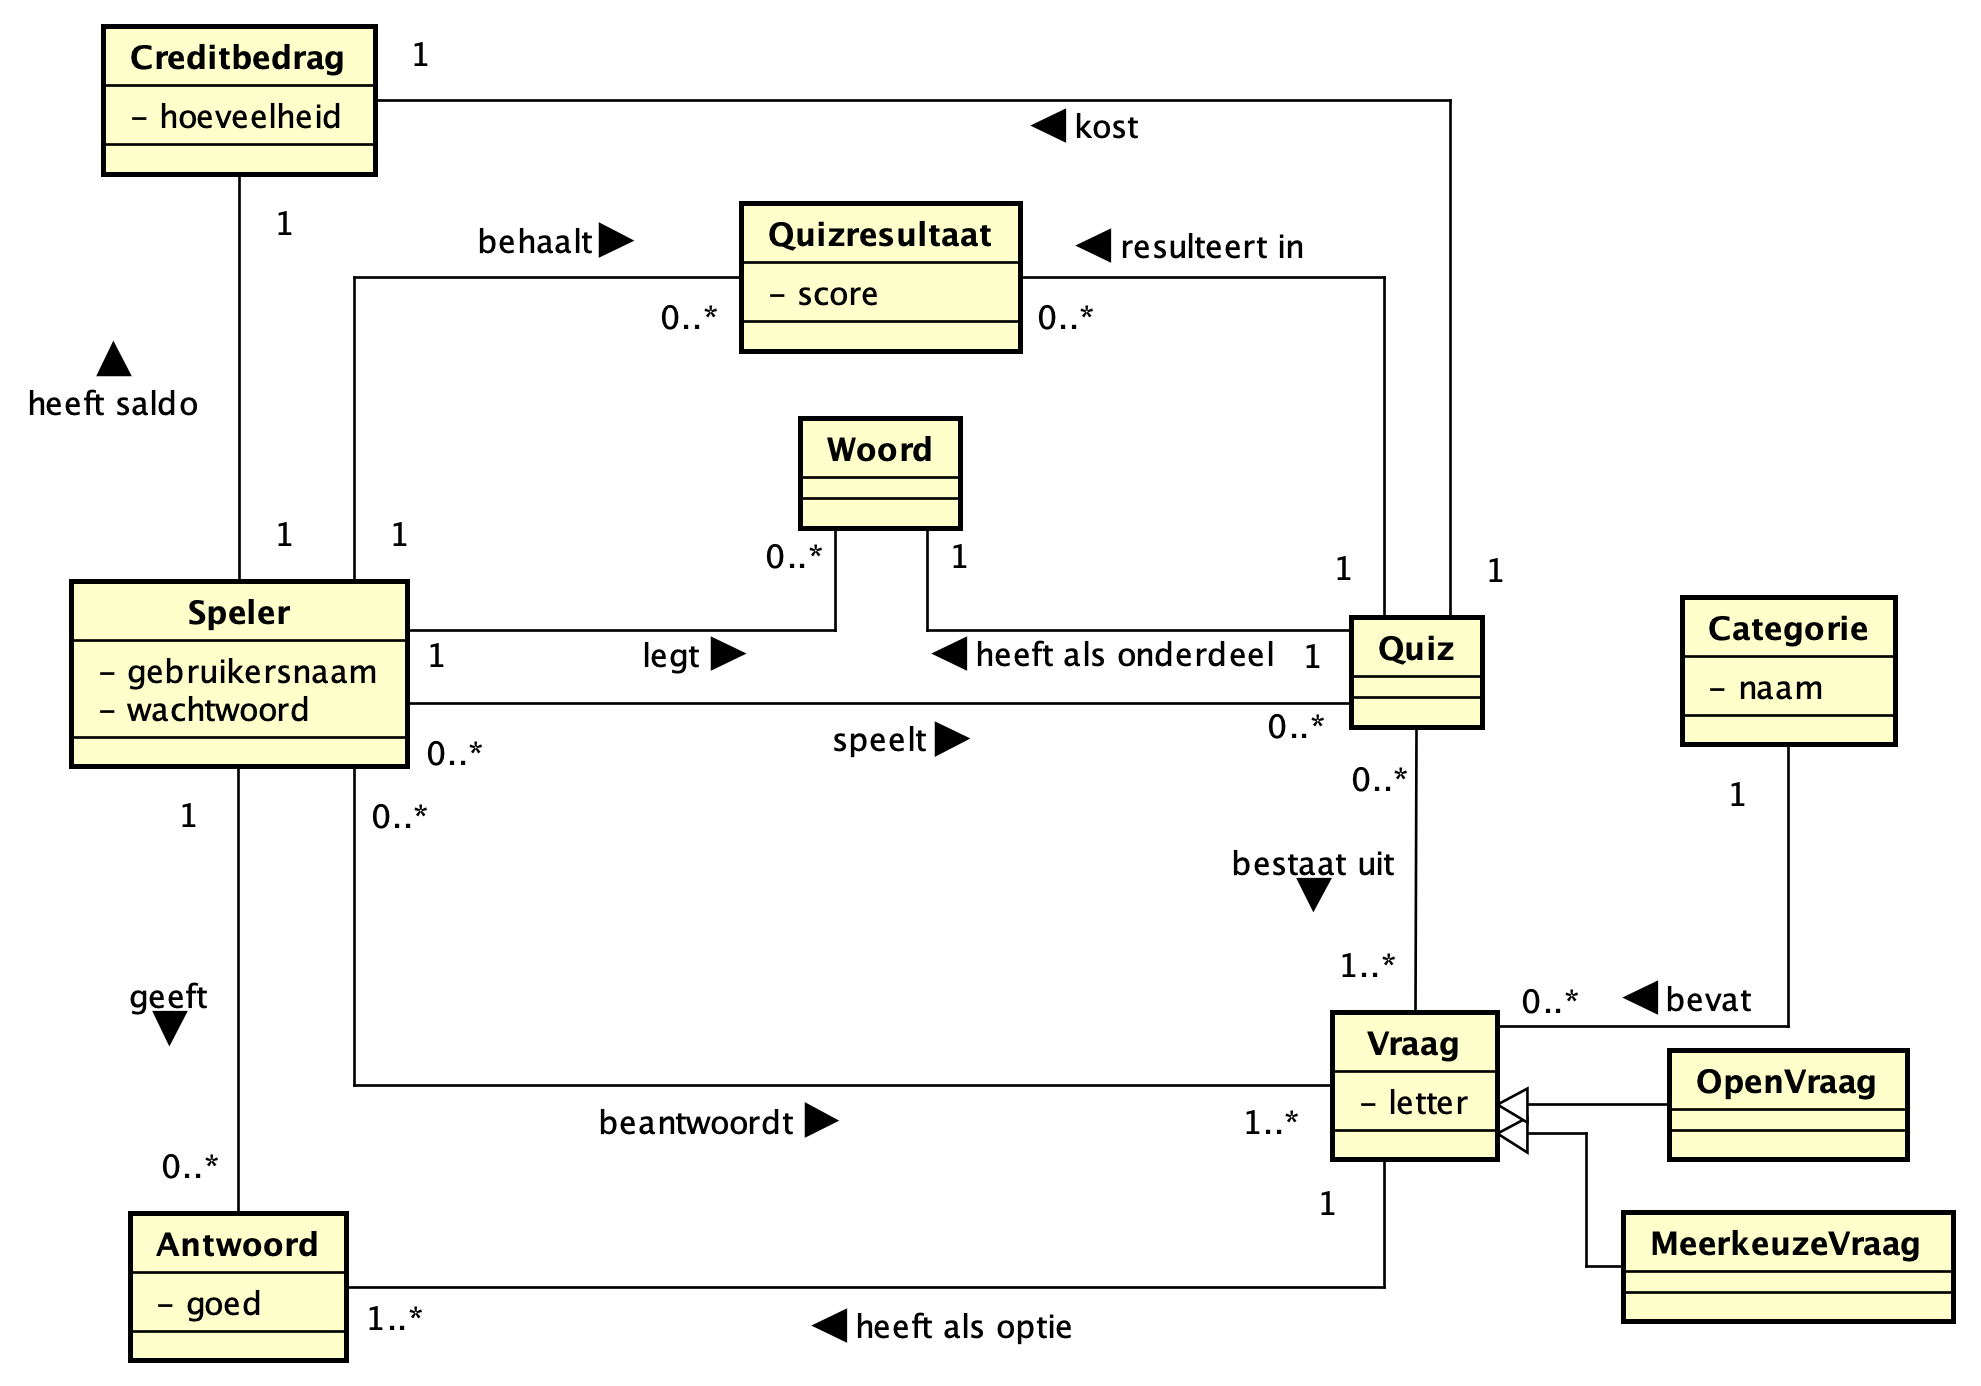
\includegraphics[width=\linewidth]{../Afbeeldingen/Domeinmodel.png}
   \caption{Domeinmodel}\label{fig:domeinmodel}
\end{mpfigure}

\subsection{Woordenlijst}
Deze sectie licht de gebruikte concepttermen uit het domeinmodel in figuur \ref{fig:domeinmodel} toe:
\begin{itemize}
   \item \textbf{Speler:} Speelt een quiz door vragen te beantwoorden. Beschikt over een creditbedrag als saldo om een quiz te betalen.
   \item \textbf{Creditbedrag:} Een hoeveelheid aan credits.
   \item \textbf{Quiz:} Een door de speler speelbare set aan vragen.
   \item \textbf{Quizresultaat:} Een door de speler behaald resultaat na het spelen van een quiz.
   \item \textbf{Categorie:} Een onderverdeling van vragen.
   \item \textbf{Woord:} Een woord dat de speler legt aan het einde van de quiz, gebruikmakend van de letters die hij door het correct beantwoorden van de voorafgaande vragen heeft verkregen.
   \item \textbf{Vraag:} Een vraag die de speler beantwoordt wanneer deze onderdeel is van een quiz.
         \begin{itemize}
            \item \textbf{OpenVraag:} Een vraag die één of meerdere goede antwoorden heeft, maar waarvan deze antwoorden niet zichtbaar zijn voor de speler.
            \item \textbf{MeerkeuzeVraag:} Een vraag die meerdere antwoorden bevat, waarvan er maar één juist is, en waarvan alle antwoorden zichtbaar zijn voor de speler.
         \end{itemize}
   \item \textbf{Antwoord:} Een mogelijk antwoord dat de speler kan geven op een gestelde vraag.
\end{itemize}

\subsection{Onderbouwing}
Deze sectie onderbouwt de gemaakte keuzes van het domeinmodel in figuur \ref{fig:domeinmodel}.

Quizzes binnen Quebble worden gespeeld door de \textbf{speler}. Om aan een \textbf{quiz} te beginnen zijn moet de \textbf{speler} geregistreerd en ingelogd zijn, en over een bepaald saldo beschikken (zie precondities uit tabel \ref{tab:usecasequizspelen}). Daarom heeft de \textbf{speler} attributen voor de inloggegevens, en beschikt hij over een bepaald \textbf{creditbedrag} als saldo. Dit saldo en de inloggegevens zijn ook vereist bij de usecases \textit{registreren} (zie sectie \ref{sec:usecaseregistreren}) en \textit{credits bijkopen} (zie sectie \ref{sec:usecasecreditsbijkopen}). De \textbf{speler} beschikt nu over de benodigdheden om een \textbf{quiz} te kunnen spelen.

Wanneer een \textbf{speler} een \textbf{quiz} start, betaalt hij eerst het \textbf{creditbedrag} wat de \textbf{quiz} kost. Een \textbf{quiz} bestaat allereerst uit een set \textbf{vragen}. Deze vragen zijn ingedeeld in \textbf{categorieën}. De \textbf{speler} geeft een voor een \textbf{antwoord} op deze \textbf{vragen}.

Wanneer het een \textbf{open vraag} betreft, zijn er één of meerdere \textbf{antwoorden} goed. Deze laten zich echter niet zien aan de \textbf{speler}.

Wanneer het een \textbf{meerkeuzevraag} betreft, is er maar één goed \textbf{antwoord}. Deze laat zich, samen met een aantal foute \textbf{antwoorden}, wél zien aan de speler.

Voor elke \textbf{vraag} die de \textbf{speler} goed beantwoordt, krijgt de \textbf{speler} een letter. Deze letters gebruikt de \textbf{speler} aan het einde van de \textbf{quiz} om een \textbf{woord} te leggen. Wanneer de \textbf{speler} een correct woord heeft gemaakt van de letters, krijgt de speler van de \textbf{quiz} een \textbf{quizresultaat}. Hierin is de berekende score te zien.

\clearpage\section{Usecasebeschrijvingen}
%Use case descriptions <In this section, each use-case is described in detail, optionally accompanied by a system sequence diagram (SSD) and operation contracts. Make sure that the use case descriptions are consistent with the domain model and the use case diagram from Section 1.5>
Dit hoofdstuk bevat uitgebreide uitwerkingen van de usecases.

De uitwerkingen bevatten fully-dressed usecasebeschrijvingen volgens de usecases.org methode (\cite[50]{larman}). Het succesvolle hoofdscenario is ingedeeld in twee kolommen als voorgesteld door \textcite{wirfsbrock}, ten behoeve van de overzichtelijkheid.

De uitwerkingen bevatten ook systemsequencediagrammen volgens \textcite{larman} die de succesvolle hoofdscenario's beschrijven \pnotecite[110]{larman}.

Eventuele activitydiagrammen zijn terug te vinden in de Software Design Description.

Alleen de drie belangrijkste usecases die nodig zijn om een quiz te spelen zijn hieronder uitgewerkt. Deze zijn geprioriteerd en verantwoord:
\begin{enumerate}
   \item \textbf{Quiz spelen:} Deze usecase bevat het gehele spelverloop voor de speler.
   \item \textbf{Registreren:} Deze usecase faciliteert precondities \textit{"Speler is ingelogd"} en \textit{"Speler is geregistreerd"} voor \textit{Quiz spelen} (zie tabel \ref{tab:usecasequizspelen}).
   \item \textbf{Credits bijkopen:} Deze usecase faciliteert de preconditie \textit{"Speler beschikt over 40 of meer credits"} voor \textit{Quiz spelen}.
\end{enumerate}
De overige usecases zijn niet essentiëel voor het spelen van het spel. Binnen de context van de opdracht, faciliteert de gemockte dataset de preconditie \textit{"Er is een speelbare quiz in het systeem aanwezig"} voor \textit{Quiz spelen}.

\clearpage\subsection{Quiz spelen}
%<Don’t really say “Use case 1.” State the use-case name instead.>

\subsubsection{Fully-dressed usecasebeschrijving}
%<Provide a fully-dressed use-case description in the format you know from the OOAD course>

\begin{xltabular}{\textwidth}{ X }
   \caption{Fully-dressed usecasebeschrijving van \textit{Quiz spelen}} \label{tab:usecasequizspelen} \\ \hline \endfirsthead\endhead
   \hspace*{\fill}\textit{Wordt vervolgd op de volgende pagina.} \\ \hline \endfoot\endlastfoot

   \textbf{Primaire actor:} Speler                  \\

   \hline

   \begin{minipage}[t]{\linewidth}
      \textbf{Stakeholders en belangen:}
      \begin{smallitemize}
         \item \textbf{Speler:} Wil een quiz spelen met zo min mogelijk eerder door hem gespeelde vragen. Wil aan het einde van de quiz zijn behaalde resultaten zien.
         \item \textbf{Bedrijf:} Wil een dermate leuke ervaring bieden aan de speler dat de speler naderhand meer credits blijft kopen.
         %\item \textbf{Medewerker:} Wil de resultaten van de gespeelde quizzes kunnen inzien, om de quizvragen zo nodig te kunnen verbeteren.
      \end{smallitemize}
   \end{minipage} \\

   \hline

   \begin{minipage}[t]{\linewidth}
      \textbf{Precondities:}
      \begin{smallitemize}
         \item Speler is geregistreerd.
         \item Speler is ingelogd.
         \item Speler beschikt over 40 of meer credits.
         \item Er is een speelbare quiz in het systeem aanwezig.
      \end{smallitemize}
   \end{minipage} \\

   \hline

   \begin{minipage}[t]{\linewidth}
      \textbf{Postcondities:}
      \begin{smallitemize}
         \item Speler heeft alle quizvragen beantwoord.
         \item Speler heeft een woord gelegd.
         \item Speler heeft zijn behaalde score gezien.
         \item Speler beschikt over 40 minder credits dan voor het spelen.
      \end{smallitemize}
   \end{minipage} \\

   \hline

   \textbf{Succesvol hoofdscenario:}

   {\begin{tabularx}{\linewidth}{ XX }
         \textbf{Actoractie}                            & \textbf{Systeemverantwoordelijkheid}                                                        \\

         \hline

         \usecasestep{Speler start een nieuwe quiz.}    &                                                                                             \\
                                                        & \usecasestep{Systeem schrijft 40 credits van de speler af.}                                 \\
                                                        & \usecasestep{Systeem laat een korte uitleg van het spelverloop en de vraagstellingen zien.} \\
                                                        & \usecasestep{Systeem laat een nieuwe quizvraag zien.}                                       \\
         \usecasestep{Speler beantwoordt de quizvraag.} &                                                                                             \\
         %& \usecasestep{Systeem slaat de beantwoorde vraag en antwoord op.}                                            \\
         \multicolumn{2}{c}{\textit{Herhaal stap 4 en 5 totdat de speler alle quizvragen heeft beantwoord.}}                                          \\
                                                        & \usecasestep{Systeem laat de behaalde letters zien.}                                        \\
         \usecasestep{Speler legt een woord.}           &                                                                                             \\
                                                        & \usecasestep{Systeem laat de behaalde score zien.}                                          \\
      \end{tabularx}}                     \\

   \hline

   \begin{minipage}[t]{\linewidth}
      \textbf{Alternatieve scenario's:}

      1a.\: Er is geen nog niet door de speler gespeelde quiz in het systeem aanwezig.
      \begin{enumerate}[nosep]
         \item Systeem meldt dat er geen nog niet gespeelde quizzes zijn.
         \item Speler kiest ervoor om een willekeurige, al gespeelde quiz te spelen.
               \begin{enumerate}[nosep,label=\theenumi\alph*.]
                  \item Speler kiest ervoor om te stoppen.
                        \begin{enumerate}[nosep,label=\arabic*.]
                           \item Stop.
                        \end{enumerate}
               \end{enumerate}
         \item Naar hoofdscenario stap 2.
      \end{enumerate}
      \bigskip
      1b.\:Het systeem was gecrasht terwijl nog niet alle quizvragen waren beantwoord.
      \begin{smallenumerate}
         \item Speler hervat de nog openstaande quiz.
         \item Naar hoofdscenario stap 4.
      \end{smallenumerate}
      \bigskip
      1c.\:Het systeem was gecrasht nadat alle quizvragen waren beantwoord, voordat er een woord was gelegd.
      \begin{smallenumerate}
         \item Speler hervat de nog openstaande quiz.
         \item Naar hoofdscenario stap 6.
      \end{smallenumerate}
      \bigskip
      5a.\:Het gegeven antwoord is leeg, of het gegeven antwoord is geen keuzemogelijkheid.
      \begin{smallenumerate}
         \item Systeem laat een foutmelding zien.
         \item Naar hoofdscenario stap 5.
      \end{smallenumerate}
      \bigskip
      7a.\:Het gegeven woord is leeg, of het woord bevat letters die niet behaald zijn.
      \begin{smallenumerate}
         \item Systeem laat een foutmelding zien.
         \item Naar hoofdscenario stap 7.
      \end{smallenumerate}
   \end{minipage} \\

   \hline

\end{xltabular}

\subsubsection{Systemsequencediagram}
%System sequence diagram (optional) <In case the use-case entails complex scenarios, you may decide to create a system sequence diagram showing events generated by external actors, the order of events and inter-system events. All systems are treated as a black box>
\begin{mpfigure}
   \centering
   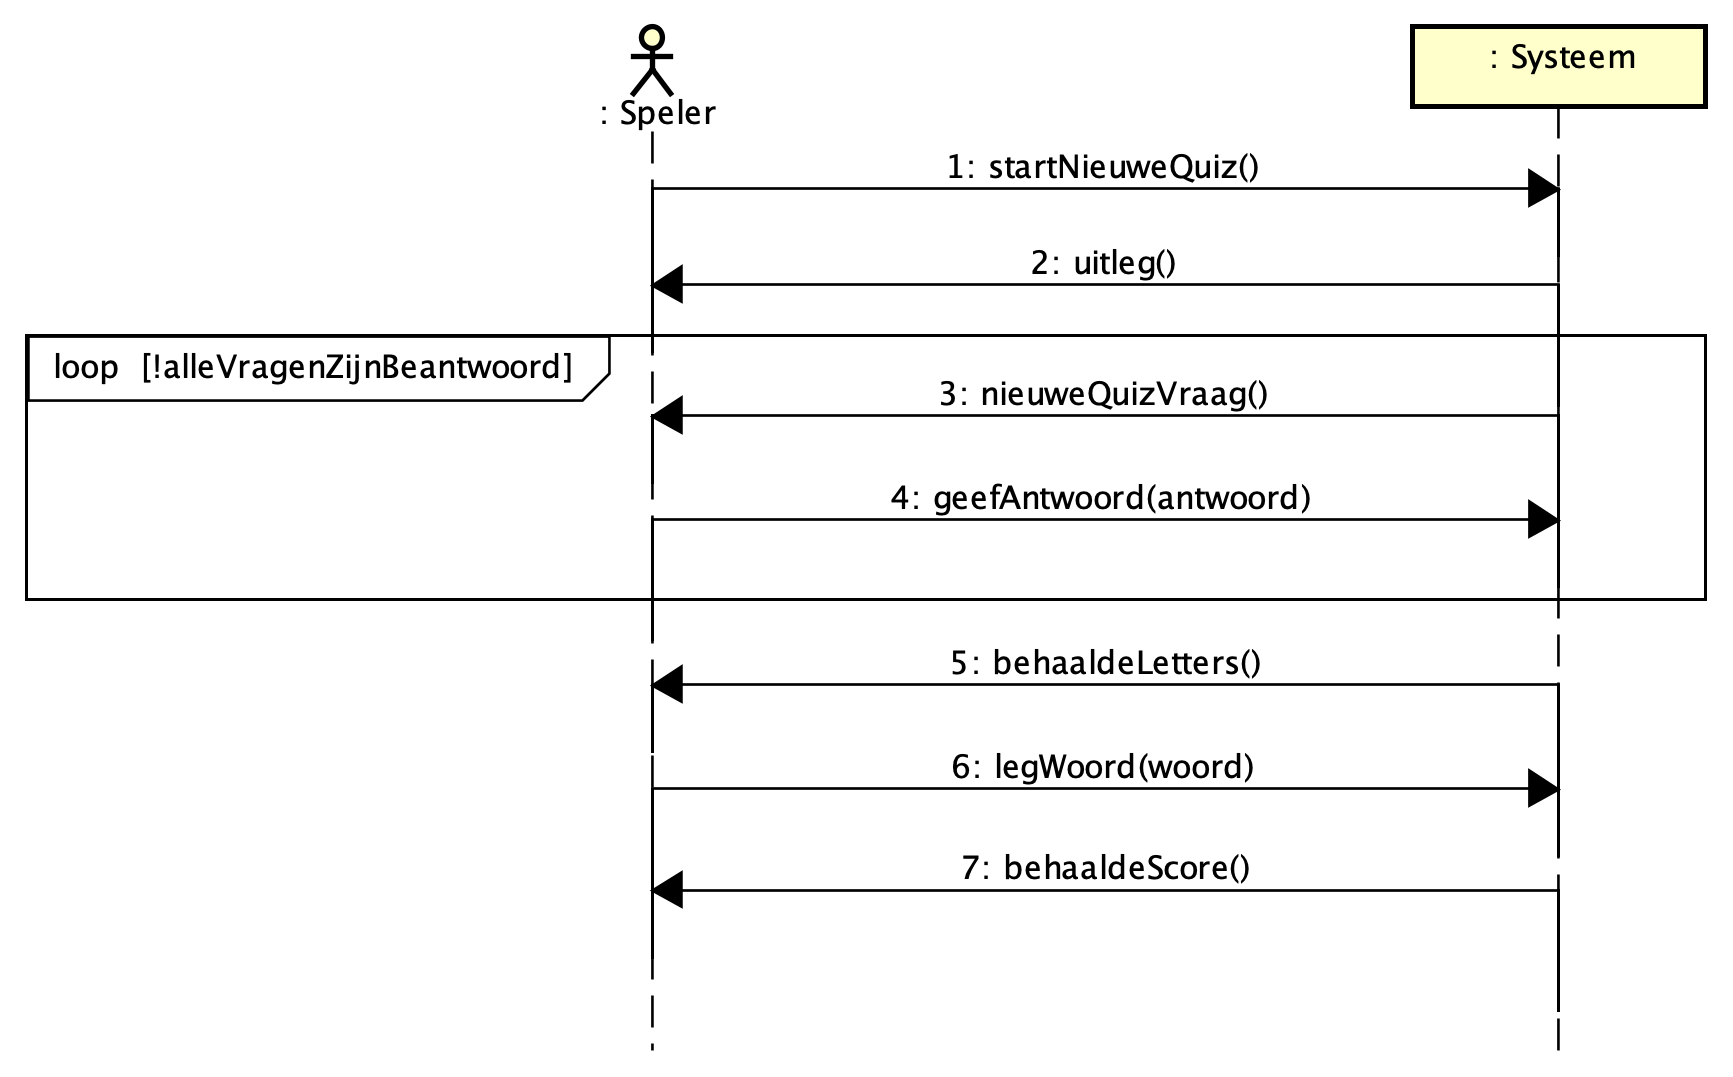
\includegraphics[width=\textwidth]{../Afbeeldingen/Quiz spelen sequence diagram.png}
   \caption{Systemsequencediagram van \textit{Quiz spelen}} \label{fig:quizspelensequencediagram}
\end{mpfigure}

\begin{landscape}
   \subsubsection{Activitydiagram}
   %haal dit weg, hoort in het SDD
   \begin{mpfigure}
      \centering
      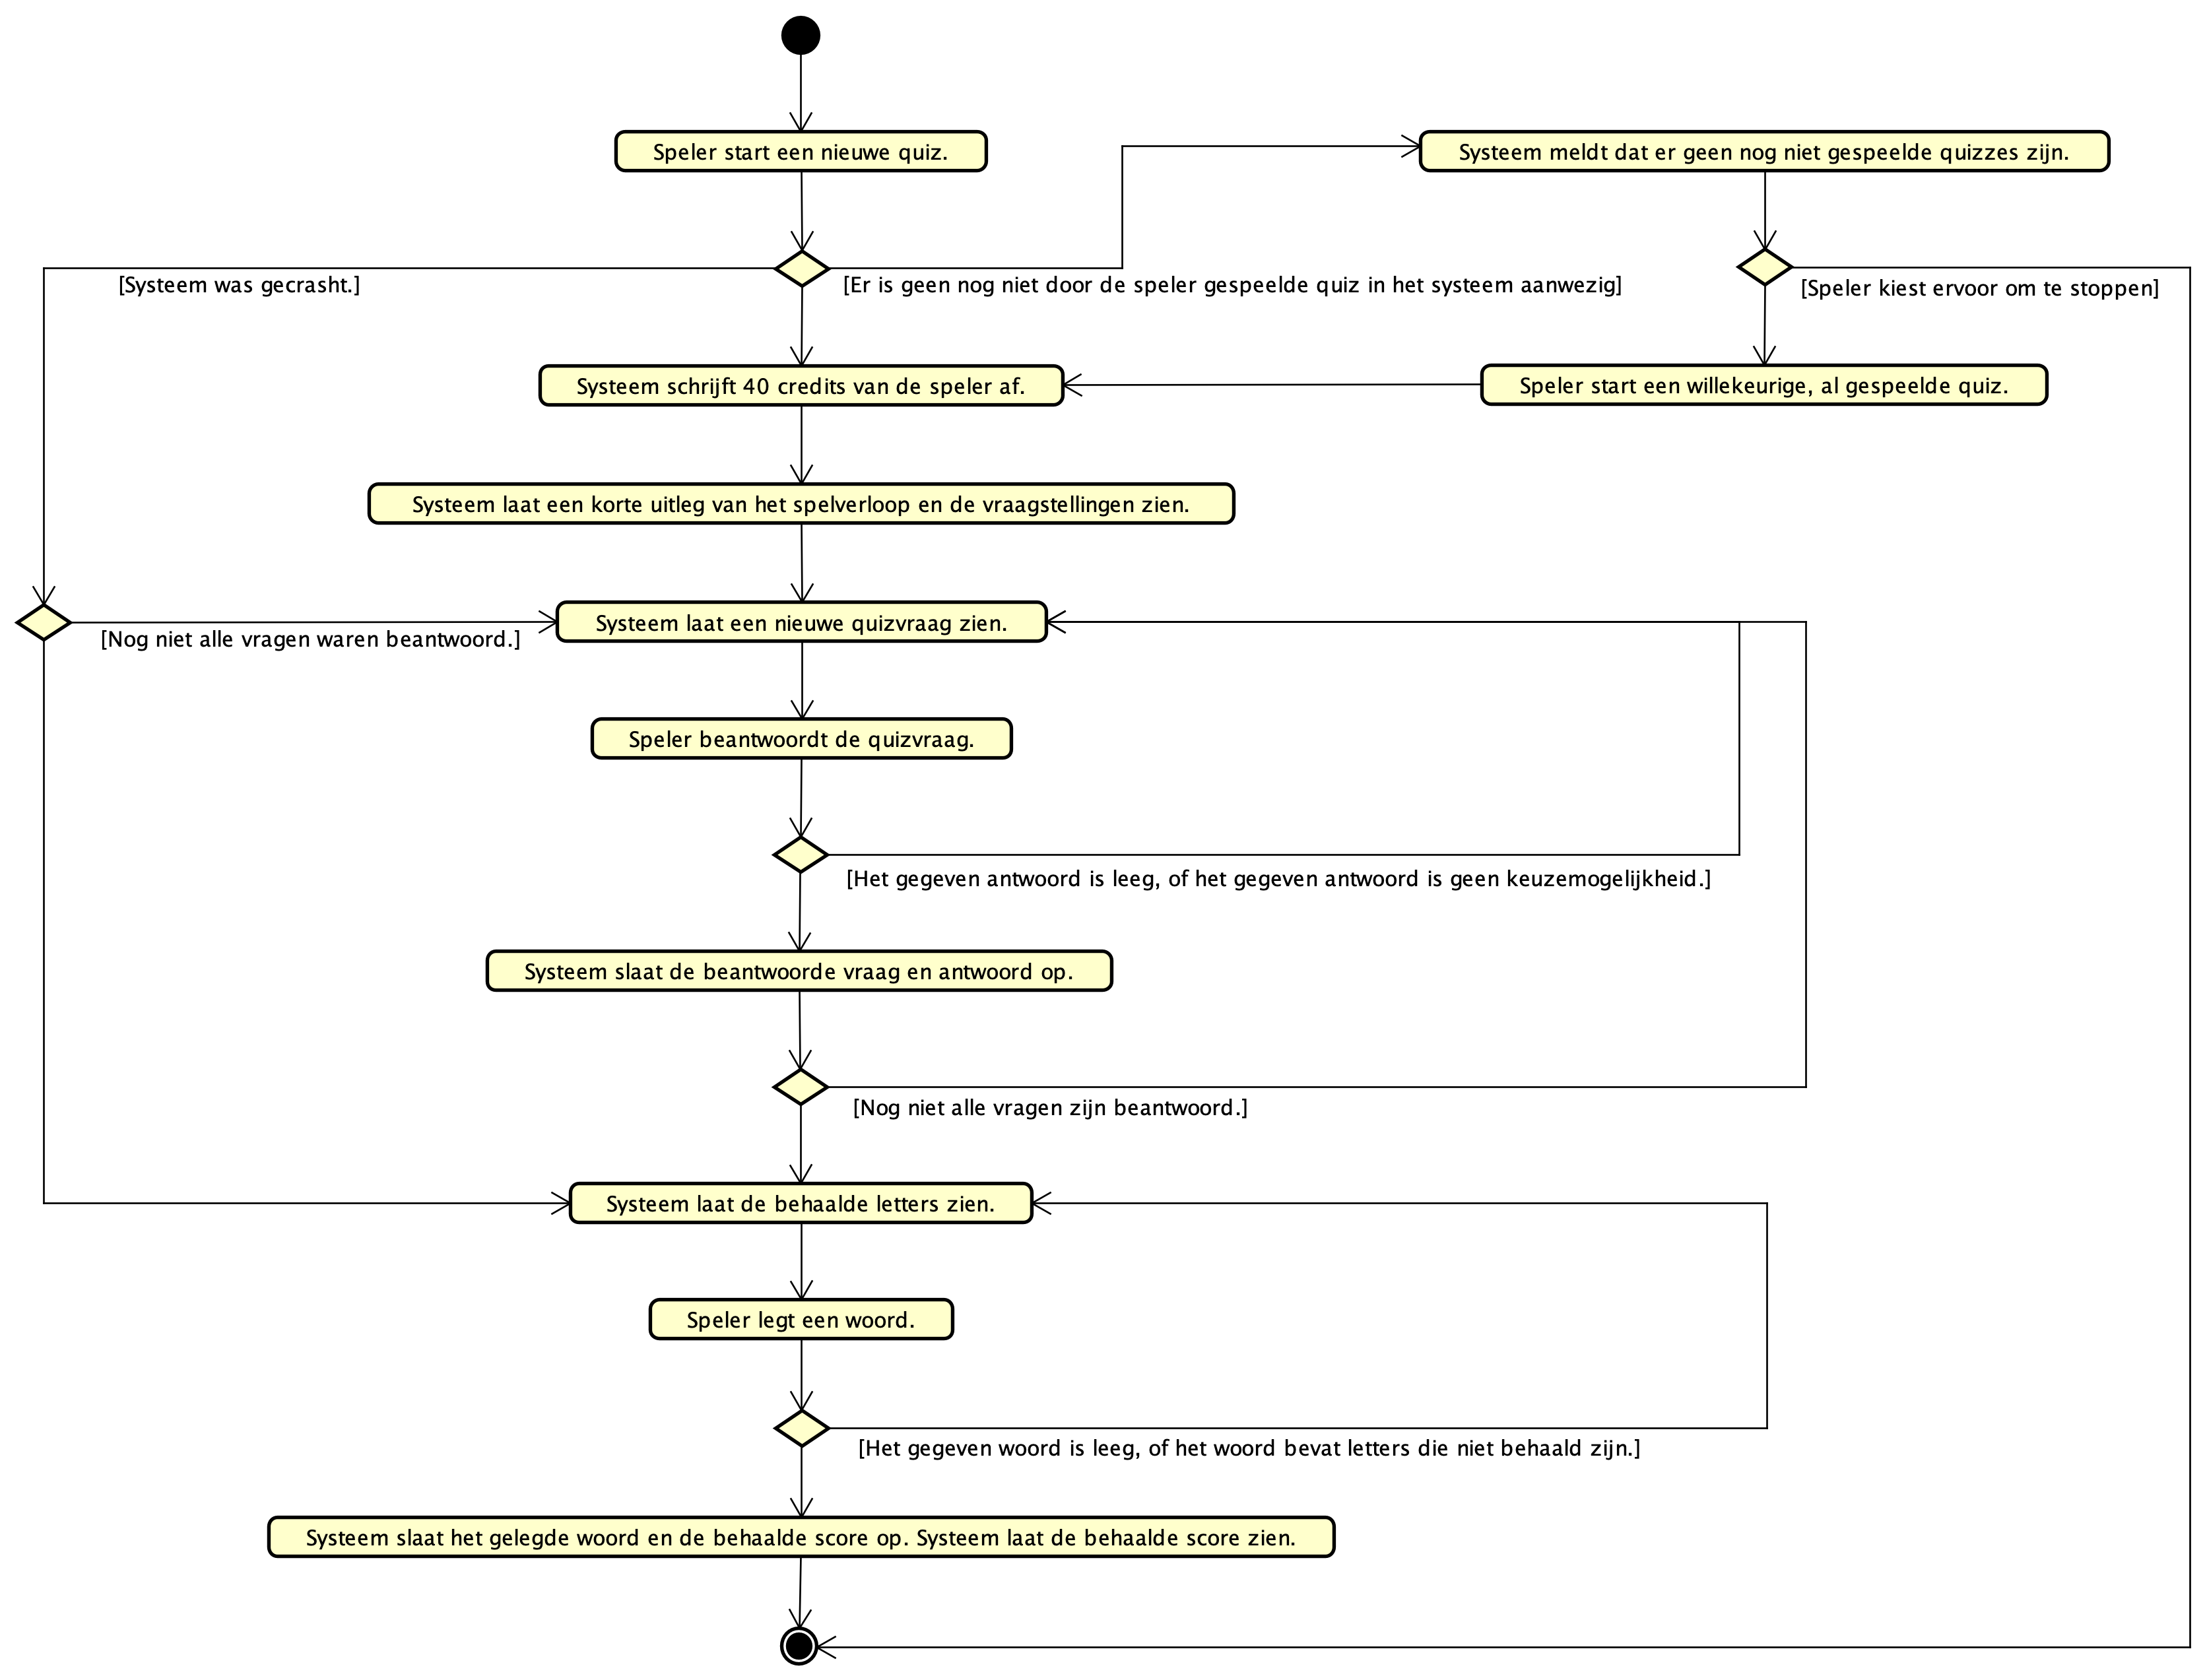
\includegraphics[scale=0.37]{../Afbeeldingen/Quiz spelen activity diagram.png}
      \caption{Activitydiagram van \textit{Quiz spelen} (wordt verplaatst naar het SDD)} \label{fig:adquizspelen}
   \end{mpfigure}
\end{landscape}

%\subsubsection{Operation contracts (optional)}
%<If the use case contains complex manipulations of domain objects, you may decide to specify operation contracts for all system operations included in the use case/ SSD.>

\clearpage\label{sec:usecaseregistreren}\subsection{Registreren}

\subsubsection{Fully-dressed usecasebeschrijving}
%<Provide a fully-dressed use-case description in the format you know from the OOAD course>
\begin{xltabular}{\textwidth}{X}
   \caption{Fully-dressed usecasebeschrijving van \textit{Registreren}} \label{tab:usecaseregistreren} \\ \hline \endfirsthead\endhead
   \hspace*{\fill}\textit{Wordt vervolgd op de volgende pagina.} \\ \hline \endfoot\endlastfoot

   \textbf{Primaire actor:} Speler                  \\

   \hline

   \begin{minipage}[t]{\linewidth}
      \textbf{Stakeholders en belangen:}
      \begin{smallitemize}
         \item \textbf{Speler:} Wil zo min mogelijk eerder gespeelde quizzes kunnen spelen. Wil na het registreren meteen kunnen beginnen met spelen.
         \item \textbf{Bedrijf:} Wil de speler doormiddel van 1000 gratis credits aanmoedigen om quizzes te spelen.
      \end{smallitemize}
   \end{minipage} \\

   \hline

   \begin{minipage}[t]{\linewidth}
      \textbf{Precondities:}
   \end{minipage} \\

   \hline

   \begin{minipage}[t]{\linewidth}
      \textbf{Postcondities:}
      \begin{smallitemize}
         \item Speler heeft een account waarmee hij quizzes kan spelen.
         \item Speler beschikt over 1000 credits.
      \end{smallitemize}
   \end{minipage} \\

   \hline

   \begin{minipage}[t]{\linewidth}
      \textbf{Succesvol hoofdscenario:}

      \begin{tabularx}{\linewidth}{XX}
         \textbf{Actoractie}                                            & \textbf{Systeemverantwoordelijkheid}                                                    \\
         \hline
         \usecasestep{Speler kiest ervoor om zich te registreren.}      &                                                                                         \\
         \usecasestep{Speler vult een gebruikersnaam en wachtwoord in.} &                                                                                         \\
                                                                        & \usecasestep{Systeem registreert de speler en schrijft 1000 credits bij de speler bij.}
      \end{tabularx}
   \end{minipage} \\

   \hline

   \begin{minipage}[t]{\linewidth}
      \textbf{Alternatieve scenario's:}

      2a.\:De gebruikersnaam is leeg, voldoet niet aan de eisen voor een gebruikersnaam, of is al geregistreerd.
      \begin{smallenumerate}
         \item Systeem laat een foutmelding zien.
         \item Naar hoofdscenario stap 2.
      \end{smallenumerate}
      \bigskip

      2b.\:Het wachtwoord is leeg, of voldoet niet aan de eisen voor een wachtwoord.
      \begin{smallenumerate}
         \item Systeem laat een foutmelding zien.
         \item Naar hoofdscenario stap 2.
      \end{smallenumerate}
   \end{minipage} \\

   \hline

\end{xltabular}

\subsubsection{Systemsequencediagram}
%<In case the use-case entails complex scenarios, you may decide to create a system sequence diagram showing events generated by external actors, the order of events and inter-system events. All systems are treated as a black box>
\begin{mpfigure}
   \centering
   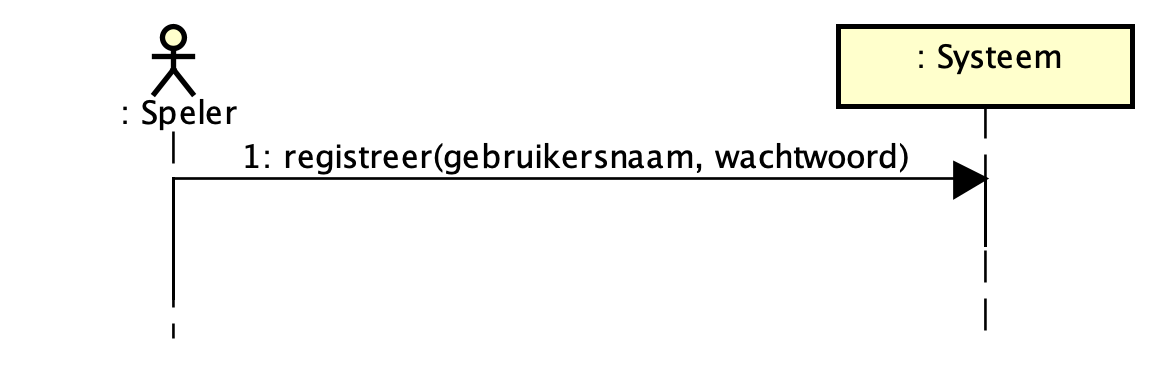
\includegraphics[width=\linewidth]{../Afbeeldingen/Registreren sequence diagram.png}
   \caption{Systemsequencediagram van \textit{Registreren}} \label{fig:ssdregistreren}
\end{mpfigure}

%\subsubsection{Operation contracts (optional)}
%<If the use case contains complex manipulations of domain objects, you may decide to specify operation contracts for all system operations included in the use case/ SSD.>

\clearpage\label{sec:usecasecreditsbijkopen}\subsection{Credits bijkopen}

\subsubsection{Fully-dressed usecasebeschrijving}
%<Provide a fully-dressed use-case description in the format you know from the OOAD course>
\begin{xltabular}{\textwidth}{X}
   \caption{Fully-dressed usecasebeschrijving van \textit{Credits bijkopen}} \label{tab:usecasecreditsbijkopen} \\ \hline \endfirsthead\endhead
   \hspace*{\fill}\textit{Wordt vervolgd op de volgende pagina.} \\ \hline \endfoot\endlastfoot

   \textbf{Primaire actor:} Speler                  \\

   \hline

   \begin{minipage}[t]{\linewidth}
      \textbf{Stakeholders en belangen:}
      \begin{smallitemize}
         \item \textbf{Speler:} Wil meer quizzes kunnen spelen dan voorheen mogelijk was.
         \item \textbf{Bedrijf:} Wil winst maken door de geldtransactie van de speler.
      \end{smallitemize}
   \end{minipage} \\

   \hline

   \begin{minipage}[t]{\linewidth}
      \textbf{Precondities:}
      \begin{smallitemize}
         \item Speler is geregistreerd.
         \item Speler is ingelogd.
      \end{smallitemize}
   \end{minipage} \\

   \hline

   \begin{minipage}[t]{\linewidth}
      \textbf{Postcondities:}
      \begin{smallitemize}
         \item Speler beschikt over het door de speler gekozen aantal credits meer dan voorheen.
         \item Speler kan de gekochte credits gebruiken om een quiz te spelen.
         \item Het bedrijf heeft de geldtransactie voor het gekozen aantal credits van de speler ontvangen.
      \end{smallitemize}
   \end{minipage} \\

   \hline

   \begin{minipage}[t]{\linewidth}
      \textbf{Succesvol hoofdscenario:}

      \begin{tabularx}{\linewidth}{XX}
         \textbf{Actoractie}                                     & \textbf{Systeemverantwoordelijkheid}                                                        \\
         \hline
         \usecasestep{Speler geeft aan credits te willen kopen.} &                                                                                             \\
                                                                 & \usecasestep{Systeem laat de mogelijke aantallen en de bijbehorende prijzen zien.}          \\
         \usecasestep{Speler kiest een aantal credits.}          &                                                                                             \\
         \usecasestep{Speler betaalt het voorgestelde bedrag.}   &                                                                                             \\
                                                                 & \usecasestep{Systeem schrijft het door de speler gekozen aantal credits bij de speler bij.}
      \end{tabularx}
   \end{minipage} \\

   \hline

   \begin{minipage}[t]{\linewidth}
      \textbf{Alternatieve scenario's:}

      3a.\:Speler annuleert het bijkopen.
      \begin{smallenumerate}
         \item Stop.
      \end{smallenumerate}
      \bigskip

      4a.\:Betaling mislukt.
      \begin{smallenumerate}
         \item Systeem laat een foutmelding zien.
         \item Naar hoofdscenario stap 2.
      \end{smallenumerate}
   \end{minipage} \\

   \hline

\end{xltabular}

\subsubsection{Systemsequencediagram}
%<In case the use-case entails complex scenarios, you may decide to create a system sequence diagram showing events generated by external actors, the order of events and inter-system events. All systems are treated as a black box>
\begin{mpfigure}
   \centering
   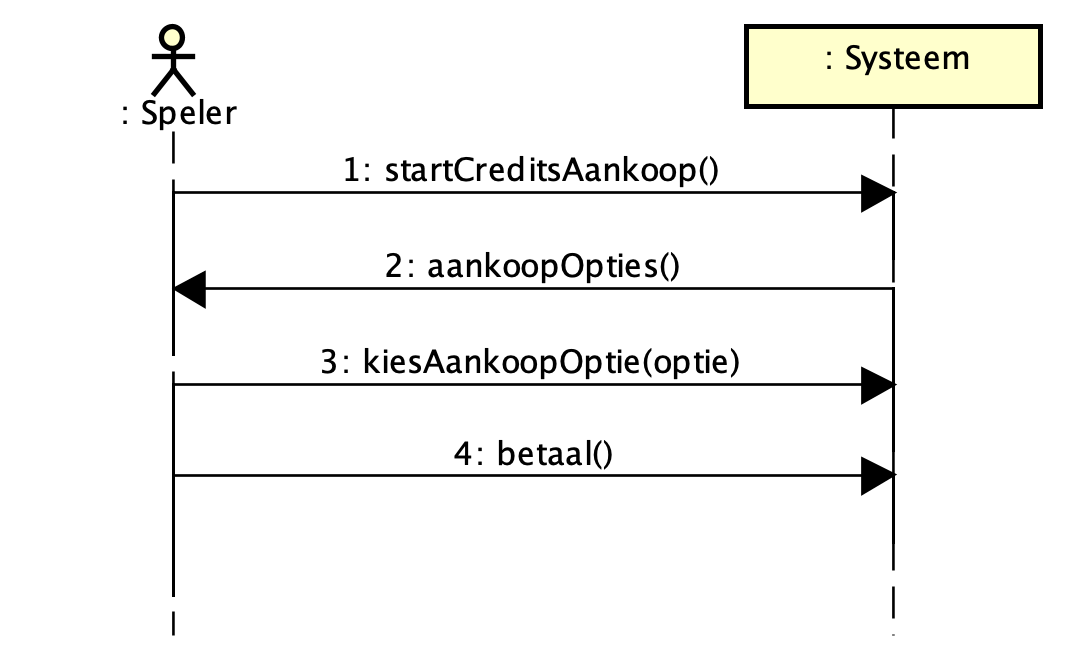
\includegraphics[width=\linewidth]{../Afbeeldingen/Credits bijkopen sequence diagram.png}
   \caption{Systemsequencediagram van \textit{Credits bijkopen}} \label{fig:ssdcreditsbijkopen}
\end{mpfigure}

%\subsubsection{Operation contracts (optional)}
%<If the use case contains complex manipulations of domain objects, you may decide to specify operation contracts for all system operations included in the use case/ SSD.>


\clearpage\section{Andere functionele eisen}
%Other functional requirements (optional) <Use this section to describe functional requirements that cannot be expressed in the shape of use cases, for instance because they do not concern goal-oriented interactions of an actor with the system. List as FRx>
Deze sectie beschrijft functionele eisen die niet in het usecasediagram te vinden zijn. De eisen zijn ieder voorzien van een korte verantwoording.
\begin{enumerate}[label=\textbf{FE\arabic*}.]
   \item De applicatie moet de wachtwoorden van spelers opslaan als Bcrypt hashes.
         \\ \textit{Dit verhoogt de beveiliging van gebruikersgegevens. Bcrypt is een van de meest veilige opties (\cite{bcrypt}).}
\end{enumerate}

\section{Niet-functionele eisen}
%Non-functional requirements <List as NFRx>
Deze sectie beschrijft de niet-functionele eisen volgens de FURPS+ methodiek (\cite{furpsplus}).

FURPS op zichzelf is een van de simpelste modellen, en houdt voornamelijk rekening met gebruikerseisen, en minder met de ontwikkelaarseisen (\cite[159]{furps}; \cite{softwarequalitymodels}). FURPS+ compenseert dit met extra categorieën (\cite{furpsplusibm}). FURPS+ is daarom een simpele doch alomvattende methodiek om eisen op te stellen.

De eisen zijn ieder voorzien van een korte verantwoording.

\subsection{Usability}
\begin{enumerate}[label=\textbf{NFE\arabic*}.]
   \item De applicatie moet het saldo van de speler laten zien gelijk nadat hij zich geregistreerd heeft.
         \\ \textit{De speler weet direct dat hij kan beginnen met spelen zonder eerst extra credits te hoeven kopen.}

   \item De applicatie moet het saldo van de speler laten zien voordat de speler een quiz start.
         \\ \textit{De speler kan op basis van het saldo een bewuste keuze maken om te spelen of niet.}

   \item De applicatie moet de kosten van een quiz aan de speler laten zien voordat de speler een quiz start.
         \\ \textit{De speler kan op basis van de kosten een bewuste keuze maken om te spelen of niet.}

   \item Wanneer mogelijk moet de applicatie altijd een nog niet gespeelde quiz kiezen wanneer de speler een quiz start.
         \\ \textit{De speler beleeft minder uitdaging bij al eerder gespeelde quizzes.}

   \item De applicatie moet de speler vragen om door te gaan wanneer er geen nog niet gespeelde quiz aanwezig is.
         \\ \textit{De speler krijgt zelf de keuze of hij het waardevol vindt om een al eerder gespeelde quiz te spelen.}

   \item De applicatie moet aan het begin van elke quiz melden dat de speler niet terug kan naar een vorige vraag.
         \\ \textit{De speler moet dit weten voor een eerlijk spelverloop.}

   \item De applicatie moet aan het begin van elke quiz een tekst laten zien waarin de vraagstelling en de antwoordmogelijkheden van de meerkeuzevragen en de open vragen uitgelegd worden.
         \\ \textit{De speler moet dit weten voor een eerlijk spelverloop.}

   \item De applicatie mag bij het controleren van antwoorden geen onderscheid maken tussen hoofdletters en kleine letters.
         \\ \textit{Dit beperkt het foutief afkeuren van goede antwoorden.}

   \item De applicatie moet aan het einde van een quiz de behaalde score laten zien aan de speler.
         \\ \textit{De speler krijgt direct inzicht in zijn prestaties, en dit kan motiveren om door te spelen.}

   \item Wanneer een speler kiest om credits te kopen, moet de applicatie de bijbehorende prijzen laten zien.
         \\ \textit{Dit voorkomt onverwachte kosten voor de speler.}

   \item De applicatie moet de speler om bevestiging vragen bij elke door de speler ge\-ï\-ni\-ti\-eer\-de transactie van credits of geld.
         \\ \textit{Dit voorkomt onverwachte kosten voor de speler.}
\end{enumerate}

\subsection{Reliability}
\begin{enumerate}[resume*]
   \item Het wijzigen van quizzes of vragen mag geen invloed hebben op quizzes die op dat moment gespeeld worden.
         \\ \textit{Dit voorkomt consistentiefouten bij quizzes die gespeeld worden (zoals dubbele vragen).}

   \item Wanneer de applicatie is gecrasht tijdens een active quiz, moet de speler deze quiz na het herstarten van de applicatie kunnen hervatten.
         \\ \textit{Dit voorkomt dat spelers hun quiz niet kunnen afmaken, en dat ze onterecht credits kwijt zijn.}
\end{enumerate}

\subsection{Performance}
\begin{enumerate}[resume*]
   \item De vertraging in de user interface nadat een speler een vraag beantwoordt mag niet langer duren dan 500 milliseconden.
         \\ \textit{Dit is een balans tussen een veilige marge voor ontwikkelaars, en een reactietijd ($<1$ seconde) die gebruikers niet als onprettig zullen ervaren (\cite[134]{usability}).}
\end{enumerate}

\subsection{Supportability}
\begin{enumerate}[resume*]
   \item De user interface, vragen en antwoorden moeten volledig vertaalbaar zijn naar andere talen.
         \\ \textit{Dit maakt het mogelijk om de applicatie uit te brengen in andere landen dan Nederland.}

   \item Het moet mogelijk zijn om extra methodes toe te voegen voor het toekennen van scores.
         \\ \textit{De uiteindelijke puntentelling ligt volgens de opdrachtgever nog niet vast.}

   \item Een externe library moet de door de speler ingevulde woorden kunnen controleren.
         \\ \textit{Hierdoor kan de applicatie gebruik maken van reeds bestaande systemen die door onder andere WordFeud en Scrabble worden gebruikt.}
\end{enumerate}

\subsection{+}
\begin{enumerate}[resume*]
   \item De applicatie moet een Java-applicatie zijn.
         \\ \textit{Java-applicaties werken op Windows, macOS, Linux, Android en, met een omweg, op iOS (\cite{oracle}; \cite{androidfundamentals}; \cite{multios}).}
\end{enumerate}

%\clearpage\section{User interface sketches (optional)}
%<Provide low-fidelity user interface sketches. Map the sketches to use cases and other requirements if applicable.>

\clearpage\printbibliography[heading=bibintoc]

\end{document} % Einde document
